\makeatletter                                                   
\def\input@path{{../}}                                          
\makeatother                                                    
\documentclass[../main.tex]{subfiles}                           
\begin{document}                                                
\chapter{Computational Results}
\label{ch:res}
This chapter will present the results from the following experiments:
\begin{itemize}
    \item Wild escape algorithm evaluation

    \item Heuristic evaluation and selection

    \item Final composition of SCALNS evaluation

\end{itemize}

Before going into the experimental results we will describe the experimental setup.
This icludes the techical side aswell as the setup of the analytical experiments themselves.
After that we will explain the generation ofthe instances used in the evaluation sections.

\section{Experimental Setup}
\label{sec:setup}
In this section we describe the technical setup of the experiments aswell as the Analytical setup of our eperiments.
\subsection{Technical Setup}
\label{sec:tech}
The computational experiments in this paper is run on two different computers. 
The more demanding experiments are run on a 64-bit Windows 10 computer with a 3.4 Ghz i7-6700 quad core processor and 16GB RAM. 
We will shorten the name of this computer to "Windows computer". 
The less demanding experiments are run on a 64-bit Ubuntu 18.04 computer with a 1.8 Ghz quad core i7-8550u processor and 16GB RAM. 
We call this computer for short "Ubuntu computer".
As a general rule through the rest of this paper; if not specified, the results were run on the Ubuntu computer.

The instance generator described in the next section was implemented in Java (version number).
The mathematical model from section 2 is setup in AMPL (version number), using the Gurobi solver. 
All AMPL experiments were run on the Windows computer.
The ALNS heuristics are implemented in Java version 10.0.4+13.
These experiments were run partly on the Ubuntu and partly on the Windows computer.
The statistical experiments are performed in Matlab R2019a version 9.6.0.1174912 on the Ubuntu computer.


\subsection{Analytics Setup}
\label{sec:analy}
In section 3 we described seven operators, aswell as a wild operator, some invented in this paper and others based on known ALNS heuristics. 
For our testing we generated five instance sets of each five instances, totally 25 instance.
While testing the algorithm from \fref{sec:wild}, we used one instance set. 
All tests were run 10 times and results are given as an average and best objective value over the 10 runs aswell as an average running time over the runs.
To analyse the performance of each of the heuristics, 5 reasonably sized instances was solved 10 times using each of the $2^7 = 128$ combinations of operators.
These $2^7=128$ runs were done on the Windows computer. \par
To determine which of the heuristics influence the result we have performed several statistical tests, including ANOVA (III) and multiple linear regression analysis, and pairwise t-tests. 
For all statistical tests in this paper we have used a $95\%$ confidence interval.
After the analysis of the heuristics, a final composition was chosen for further testing.
We then compared the performance of the final composition with solutions found by the mathematical model in AMPL. We also present figures which show the performance of our selected heuristics in a hphazardly selected single run.

For these tests we compare the results toward the best known solution from AMPL and ..... TODO.
We use a $95\%$ confidence level for all statistical experiments in this paper.

\section{Instances}
\label{sec:ins}
The instance generator was created based on real data from an anonumous costomer of 4flow. 
Following, we will describe how we designed the generator and how we generated the instances used in the analytical part of the paper.

\subsection{Generate Instances based on real data}
\label{sec:data}
The 4flow data gives information about the number of orders $|N|$, locations $|L|$, factories $|F|$. 
The amount of vehicles $|V|$ are kept large compared to the amount of orders to make sure there are enough but not too many vehicles. 
A solution that uses all but one vehicle is the ideal here and we found $|N|/2 \leq |V| \leq 2/3 |N|$ to be fitting.
$|N|, |V|, |L|, |F|$ are given as input to the generator.
In addition the data from 4flow gave us information about the size of a vehicle and its compatabilities. 
Some vehicles might have cooling possibilities amd some speical equipment required for transport of special goods or equipment required at the pickup or delivery location etc.).
Other information aquired by the data was travel distances, cost structure etc.

\par
To keep the instances feasible but still as realistic as possbile it makes sense to limit the data to different possibilities.
Our data was generated with the following properties:
\begin{itemize}
    \item Orders are assigned to pickup and delivery locations randomly. Orders assigned to the same location are given the same stop $L_s$
    \item Each delivery location is assigned to a factory at random $N_f$.
    \item Each location aswell as each order is assigned a special property with $5\%$ probability. This will decide which vehicle can pickup which order, $N^P_v$ and $N^D_v$
    \item We let the vehicles types be split up in 3 different vehicle types, small, medium, large, each with extected capacitied and capabilities.
        \begin{itemize}
            \item Large vehicle: slower but compatible with all locations and orders, with $Q^{kg}_v=24k$ and $Q^{vol}_v=102$
            \item Medium vehicle: medium fast and compatible with all locations but not orders with special compatability, with $Q^{kg}_v=18k$ and $Q^{vol}_v=71$ 
            \item Small vehicle: fastest but not compatible with special locations and special orders, with $Q^{kg}_v=12k$ and $Q^{vol}_v=55$ 
        \end{itemize}
    \item The distances $d_{ij}$ were calculated using pytagoras on the randomly generated points described in the next section 
    \item The travel time $T_{ijv}$ were scaled with $60\%$ of the travel distance, added with a random variation of $+/- 10\%$ of the travel distance, multiplied by the speed of the vehicle (slow: $*=105\%$, medium: $*=102.5\%$).
    \item The cost matrices $C^{km}_{v\alpha\beta}$, $C^{kg}_{v\alpha\beta}$, $C^{fix}_{v\alpha\beta}$ were based on a real 4flow cost matrix, scaled to the size of the instance and to the size of the vehicle.  
    \item The cost of no transport $C_i$ was set to a minimum lower bound scaled based on the weight/volume/distance of the order.
    \item The stop costs $C^{stop}_{vi}$ were calculated realtive to the size of the vehicle and the cost data from 4flow.
    \item Time windows $[\underline{T_{ip}},\overline{T_{ip}}]$  were generated randomly based on typical factory opening hours. 1-2 timewindows per day, and 3-7 days per week saceld based on the instance size. 
\end{itemize}

\subsubsection{Random locations based on real georaphical data}
Most of 4flow's customers are based either in Germany or in Europe. 
To make the instance generator as realistic as possible we have decided to split the instances into 3 geographical types; 
European, German and uniform geographically distributed locations.
We made 2 maps based on real scale approximations of geographical data from National Geographics, in km.
To simplify we have sticked to geographical points with an eliptic uniformly distributed area surrounding the point to represent a country or a city.
\fref{fig:areas} illustrates the areas of possible locations used in the generator. 
Larger elipses are more likely to be selected by the generator than smaller elipses.
\begin{figure}
\centering
    \caption{Area of random point generation}
    \begin{subfigure}[b]{0.3\textwidth}
        \centering
        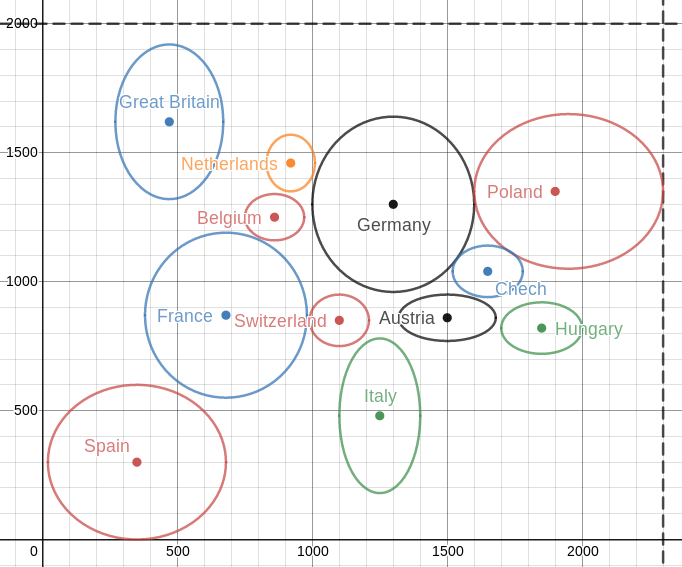
\includegraphics[width=\textwidth]{europe_coordinates}
        \caption{Europe}
        \label{fig:eur}
    \end{subfigure}
    \hfill
    \begin{subfigure}[b]{0.3\textwidth}
        \centering
        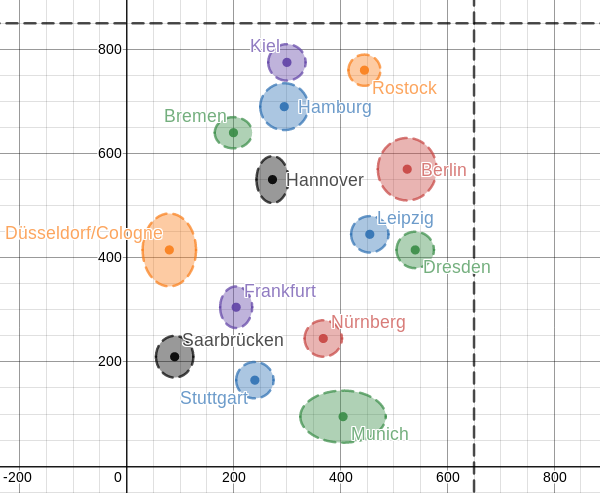
\includegraphics[width=\textwidth]{germany_coordinates}
        \caption{Germany}
        \label{fig:ger}
    \end{subfigure}
    \hfill
    \begin{subfigure}[b]{0.3\textwidth}
        \centering
        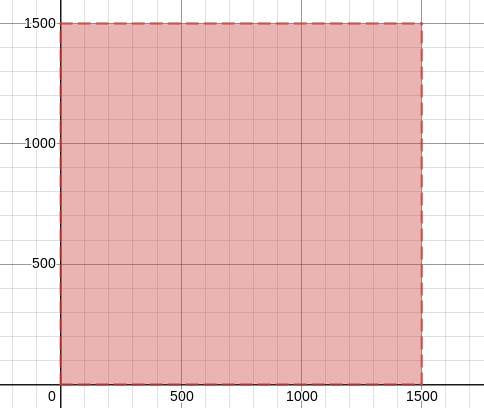
\includegraphics[width=\textwidth]{uniform_coordinates}
        \caption{Uniform}
        \label{fig:uni}
    \end{subfigure}
    \label{fig:areas}
    \caption*{Shaded areas indicate a possible location generation. Larger areas are more likely to get picked}
\end{figure}

For the selected elipse a point was selected within the elipse at random with a uniform distribution.
For \fref{fig:uni} points were generated at random within the limits shown.
From our 5 instance sets, two were generated using \fref{fig:eur}, two with \fref{fig:ger} and one with the uniform distribution from \fref{fig:uni}. 
If a point belong in the same factory as a previously generated point, that point was generated within a reasonable radius of three kilometer.

\subsection{Generated Instances}
\label{sec:geni}
For testing our algorithm in this paper, 5 instance sets of each 5 instances of varying sizes were generated. 
We have numbered the sets as follows:
\begin{itemize}
    \item Set 1 and set 2 are generated based on the European map from \fref{fig:eur}
    \item Set 3 and set 4 are generated on the german map from \fref{fig:ger}
    \item Set 5 is generated on the uniform distribution from \fref{fig:uni}
\end{itemize}

Each instance set contain representative instance sizes of our problem based on data from 4flow, $4, 12, 35, 80, 150$ orders using respectively $3, 7, 20, 45 & 80$ vehicles and containing $7, 9, 22, 45, 85$ locations.  
The sizes of the instances and the instance set number are shown for each result presented in the following sections.

\section{Initial Results}
\label{sec:res}
In this section we will present the data from our experiments. 
This data lead us to the final composition of our model.
We have done this in 3 parts:
\begin{itemize}
    \item Evaluation of wild escape algorithm
    \item Initial evaluation of heuristics
    \item Further evaluation of heuristics
\end{itemize}
In the last part of this section we will present the final composition of our model.
The results from the final composition are presented in the next section.

\subsection{Evaluation of the wild algorithm}
\label{sec:evalw}
To help our algorithm escape from a neighbourhood position we designed a wild algorithm described in section \fref{sec:wild}. To evaluate the implementaion of this operator we have decided to evaluate the result of running the complete ALNS with all heuristics included with three different modifications. 
First we run the algorithm without any escape algorithm.
Secondly we ran the algorithm with a modification that resets the algorithm each time we get stuck and start from a new random solution.
And lastly we ran our algorithm with our escape algorithm.
Comparing these three options towards eachother will help us evaluate if our wild algorithm is helping us in general and see if our wild algorithm is different than doing a reset and just starting from a new solution somewhere.

\subsubsection{Results of running ALNS}
We ran our algorithm 10x3 times, ten for each escape adjustment, on instance set 1 from \fref{sec:ins}.
We modified our escape algorithm on this run to ignore if a best solution is found while moving from one neighbourhood to the next. 
This way the extra iterations explained in \fref{sec:wild}, does not give any unfair advantage to our wild escape algorithm. We will simply be moving from one neighbourhood to the next without checking if we find a better solution on the way.
\par
The result from running our algorithm with these three adjustments are summarized in \fref{tab:wildComp}.
It shows the objective values found on average during each of the 10 runs, the best solution found overall and the average running time, for each excape adjustment.
\begin{table}
    \centering
    \caption{ALNS with all heuristics using 3 different reset algorithms}
    \begin{adjustbox}{width=\columnwidth,center}
            \begin{tabular}{|ccc|c|ccc|ccc|ccc|}
            \hline
                        &           &           & Initial           & \multicolumn{3}{c|}{Average Objective}         & \multicolumn{3}{c|}{Best Objective}            & \multicolumn{3}{c|}{Running time (sec)}   \\ 
                #Ord    & #Veh      & #Loc      & Objective         & No esc        & Rnd rst       & Wild esc      & No esc        & Rnd rst       & Wild esc      & No Esc    & Rnd rst & Wild Esc        \\
            \hline
                4       & 3         & 7         & $609\,680.3$     & $3\,444.7$   & $3\,444.7$   & $3\,444.7$   & $3\,444.7$   & $3\,444.7$   & $3\,444.7$   & $0.18$    & $0.20$    & $0.20$        \\
                12      & 7         & 9         & $1\,023\,745.5$  & $149\,692.6$ & $154\,832.9$ & $149\,692.4$ & $149\,692.4$ & $149\,692.4$ & $149\,692.4$ & $0.39$    & $0.51$    & $0.46$        \\
                35      & 20        & 22        & $2\,682\,067.9$  & $10\,639.1$  & $10\,849.5$  & $10\,350.9$  & $10\,404.9$  & $10\,358.6$  & $10\,025.1$   & $2.31$    & $1.61$    & $2.49$        \\
                80      & 45        & 45        & $6\,422\,128.6$  & $22\,262.2$  & $25\,802.9$  & $21\,377.4$  & $20\,761.2$  & $21\,777.4$  & $20\,831.3$  & $15.89$   & $8.05$    & $14.97$       \\
                150     & 80        & 85        & $12\,059\,380.3$ & $40\,667.2$  & $38\,313.0$  & $35\,705.7$  & $34\,316.0$  & $34\,345.0$  & $34\,282.3$  & $88.21$   & $48.92$   & $77.78$      \\
            \hline
            \end{tabular}
    \label{tab:wildComp}
    \end{adjustbox}
    \caption*{The columns contains in order: the first three columns show the instance size in number of orders, vehicles and locations. 
    Then follows three columns that contain the average improvement from runs with the different escape adjustments: no escape, random reset and our escape alorithm. The next three columns contain the best improvement for the same three escape adjustments, and the final three columns contain the average running time in seconds for the three escape adjustments.}
\end{table}

\subsubsection{Observations of results from wild algorithm evaluation}
The \fref{tab:wildComp} shows that on average using our wild algorithm clearly outperforms both the restart algorithm and not including a reset algorithm. 
We see that the average result for all instance sizes are lowest using our wild algorithm. 
In addition our wild algorithm outperforms the others for all instances in finding the best solution, except for the instance with 80 orders, where not using an escape algorithm ended up finding a better best solution. 
This is however probably due to the algorithm ending in a lucky neighbourhood and since the wild operator is vastly improving the solution on average we still think it is better to run our algorithm with the wild escape algorithm adjustment.
\par
With regards to the running time we observe the following pattern for the largest two instances: the random restart is the fastest, followed by our wild escape algorithm, and lastly not using any escape algorithm. It is ecspected that the random reset here outperforms the others as we have generated the random solutions before starting our algorithm. The random reset also resets the weights of all of the heuristics and that could indicate that fast heuristics get more running time here than they usually would get. Since our wild escape algorithm is clearly outperforming the others we have accepted the slight increase in runningtime.  

\subsection{Initial evaluation of heuristics}
\label{sec:evalH1}
Different heuristics have different strengths and weaknesses. Some heuristics are not performing well on their own, but work very well in combination with other heuristics. 
Other heuristics are stron on their own, and their performance is prohibited by other heuristics, or not getting enough running time when too many heuristics are included.

\par To find the right combination of heuristics we have done an evaluation of their performance to search for the best possible combination of operators. To do this selected the instance set with a representative size of ... and ran our algorithm, without the wild algorithm adaptation, with each combination of operators.
This results in $2^7 = 128$ each running 10 times. To be able to compare the results from differnt instances we calculated the improvements from the initial solution which resulted in the improvement from the best solution found during the 10 runs, and an average improvement from the initial solution from the 10 runs of each combination. Each observation was also multiplied by $1000$ to make the analysis more readable. 

\par We evaluated the data resulting from the different combination in three steps:
\begin{itemize}
    \item In the first part we ranked the combinations based on the best improvement and the average improvement
    \item In the second part we ran ANOVA and regression analysis to see which heuristics have a significant impact on the result
    \item In the third part we run t-tests to see if certain heuristics in combination with others have a positive or a negative impact on the final result
\end{itemize}

\subsubsection{Ranking the combinations}
We shorten the names of each heuristic and will refer to them for here on as components. The components are assigned the following names:
\begin{itemize}
    \item C1: this is the swap heuristic described in \fref{sec:swap}
    \item C2: exchange heuristic from \fref{sec:exch}
    \item C3: is the 2-opt heuristic in \fref{sec:2opt} 
    \item C4: is the random removal first fit insertion heuristic from \fref{sec:rand}
    \item C5: clustering heuristic described in \fref{sec:clust}
    \item C6: this is the worst removal and greedy insert heuristic in \fref{sec:greedy}
    \item C7: is the shaw removal and regret-3 insertion heuristic described in \fref{sec:shaw}
\end{itemize}

\Fref{fig:rank} shows the ranking of each combination of components from left to right.
A colored tile indicates that the current component is in use.
The further a combination is to the left, the higher improvement was from the initial solution compared to the other combinations. \par
The figure \ref{fig:avrgRank} shows the combination of components ranked based on the average improvment over the 10 runs for that combination.
Then figure \ref{fig:bestRank} shows the combination of components ranked based on the best improvement overall during the 10 runs.
Finally figure \ref{fig:avrgBestRank} shows the ranking of the average improvement + the best improvement to see which combinations performs best overall.

\begin{figure}
    \centering
    \caption{Ranking of improvements from initial solution}
    \begin{subfigure}[b]{0.95\textwidth}
        \centering
        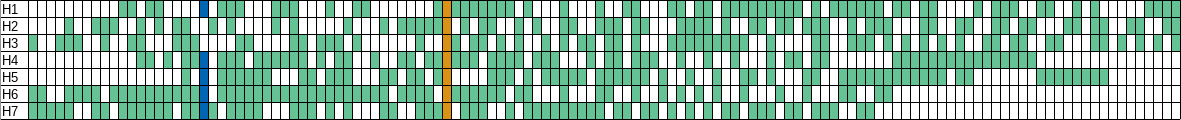
\includegraphics[width=\textwidth]{avrg_imp_rank}
        \caption{Average improvement}
        \label{fig:avrgRank}
    \end{subfigure}

    \begin{subfigure}[b]{0.95\textwidth}
        \centering
        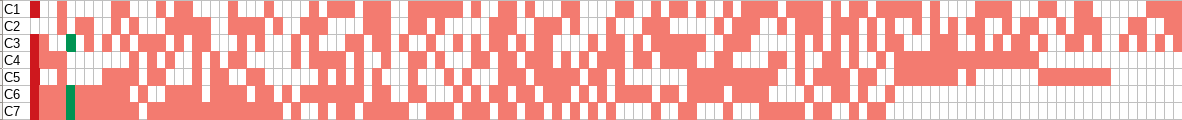
\includegraphics[width=\textwidth]{best_imp_rank}
        \caption{Best improvement}
        \label{fig:bestRank}
    \end{subfigure}

    \begin{subfigure}[b]{0.95\textwidth}
        \centering
        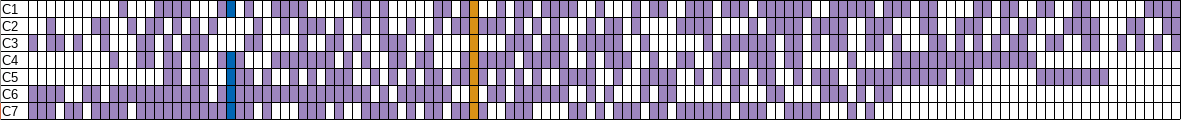
\includegraphics[width=\textwidth]{best_avrg_imp_rank}
        \caption{Best+Average improvement}
        \label{fig:avrgBestRank}
    \end{subfigure}
    \label{fig:rank}
    \caption*{Highlighted tiles indicate use of a component. The blue highlighted tiles show the final composition. Yello highlighted tiles show the use of all operators.}
\end{figure}



\subsubsection{ANOVA and regression analysis}
The ranking gives us an overview over which components are working and is always part of a good combination.
It also gives us information on which components are not performing well overall and which combination of components are not working well.
However, ANOVA and regression analysis can help us evaluate which components have a significant positive impact on the result.
\Fref{tab:anovaNormal} shows the results of ANOVA (III) analysis performed using each component as a source of variance. 
We extended the model with the instances as random effects to give us a better explanation of the result and less noise in the model. 
We did one ANOVA analysis for the average improvement over 10 runs shown in figure \ref{tab:anovaAvrgNormal}, and one for the best improvement found in figure \ref{tab:anovaBestNormal}. \par

\begin{table}
    \centering
    \caption{Analysis of variance}
    \begin{adjustbox}{width=\columnwidth,center}
        \begin{subtable}{.75\columnwidth}
            \centering
            \begin{tabular}{cccccc}
            \hline
            Source  &Sum sq.    &df &Mean sq.   &F      &P$>$F \\ 
            \hline
            C1      & 0.052     & 1 & 0.052     & 0.09  & 0.7682\\
            C2      & 0.748     & 1 & 0.748     & 1.26  & 0.2628\\
            C3      & 0.038     & 1 & 0.038     & 0.06  & 0.8017\\
            C4      & 22.432    & 1 & 22.432    & 37.66 & 0     \\
            C5      & 12.734    & 1 & 12.734    & 21.38 & 0     \\
            C6      & 117.945   & 1 & 117.945   & 198   & 0     \\
            C7      & 112.406   & 1 & 112.406   & 188.7 & 0     \\
            Instance& 371.704   & 4 & 92.926    & 156   & 0     \\
            Error   & 350.257   &588& 0.596     &       &       \\
            Total   & 975.207   &599&           &       &       \\
            \hline
            \end{tabular}
        \caption{Average improvement statistics}
        \label{tab:anovaAvrgNormal}
        \end{subtable}
        \hfill
        \begin{subtable}{.75\columnwidth}
            \centering
            \begin{tabular}{cccccc}
            \hline
            Source  &Sum sq.    &df &Mean sq.   &F      &P$>$F \\ 
            \hline
            C1      & 0.075     & 1 & 0.0745    & 0.23  & 0.6306\\
            C2      & 0.195     & 1 & 0.1949    & 0.61  & 0.4369\\
            C3      & 0         & 1 & 0.0001    & 0     & 0.988 \\
            C4      & 8.372     & 1 & 8.3718    & 26    & 0     \\
            C5      & 3.679     & 1 & 3.6789    & 11.43 & 0.0008\\
            C6      & 66.236    & 1 & 66.2357   & 205.71& 0     \\
            C7      & 67.081    & 1 & 67.0813   & 208.33& 0     \\
            Instance& 344.971   & 4 & 86.2428   & 267.84& 0     \\
            Error   & 189.331   &588& 0.322     &       &       \\
            Total   & 671.378   &599&           &       &       \\
            \hline
            \end{tabular}
        \caption{Best improvement statistics}
        \label{tab:anovaBestNormal}
        \end{subtable}
    \end{adjustbox}
    \label{tab:anovaNormal}
    \caption*{The columns contains in order: the source of the variability and for each source the sum of the sqares, the degrees of freedom, the mean squares, the F-statistic and the p-value.}
\end{table}

In addition to this we performed a multiple linear regression in \fref{tab:regrNormal} on the same data as the ANOVA.
The regressional analysis gives us insight into wether a component is positively or negatively influencing the result aswell as how well the components explain the result through the $R^2$.
Also here we used the Instances as a random effect, and the final instance is when all Instance terms are 0.

\begin{table}
    \centering
    \caption{Results of multiple linear regression model}
    \begin{adjustbox}{width=\columnwidth,center}
        \begin{subtable}{.75\columnwidth}
            \centering
            \begin{tabular}{ccccc}
            \hline
            Term    &Estimate   & SE    & tStat & pValue \\ 
            \hline                
        Intercept   & 994.58    & 0.11713       & 8491.5    & 0         \\
            C1      & -0.018582 & 0.063017      & -0.29487  & 0.7682    \\
            C2      & -0.07063  & 0.063017      & 1.1208    & 0.26283   \\
            C3      & -0.01583  & 0.063017      & -0.2512   & 0.80175   \\
            C4      & 0.39108   & 0.063729      & 6.1366    & 1.5502e-09\\
            C5      & -0.29466  & 0.063729      & -4.6236   & 4.6407e-06\\
            C6      & 0.89676   & 0.063729      & 14.071    & 5.7098e-39\\
            C7      & 0.87544   & 0.063729      & 13.737    & 1.923e-37 \\
            Inst1   & 0.50928   & 0.099639      & 5.1113    & 4.3337e-07\\
            Inst2   & -0.051052 & 0.099639      & -0.51237  & 0.60859   \\
            Inst3   & 1.6601    & 0.099639      & 16.662    & 2.4375e-51\\
            Inst4   & 1.755     &  0.099639     & 17.614    & 4.4128e-56\\
            \hline
            \end{tabular}
        \caption{Average improvement statistics, $R^2=0.641$}
        \label{tab:regrAvrgNormal}
        \end{subtable}
        \hfill
        \begin{subtable}{.75\columnwidth}
            \centering
            \begin{tabular}{cccccc}
            \hline
            Term    &Estimate   & SE    & tStat & pValue \\ 
            \hline                
        Intercept   & 994.97    & 0.086114      & 11554     & 0         \\
            C1      & 0.022291  & 0.046332      & 0.48112   & 0.63061   \\
            C2      & -0.036047 & 0.046332      & -0.77801  & 0.43687   \\
            C3      &-0.00069693& 0.046332      & -0.015042 & 0.988     \\
            C4      & 0.23891   & 0.046855      & 5.099     & 4.6112e-07\\
            C5      & -0.15838  & 0.046855      & -3.3801   & 0.00077249\\
            C6      & 0.67202   & 0.046855      & 14.342    & 3.2e-40   \\
            C7      & 0.67629   & 0.046855      & 14.434    & 1.2062e-40\\
            Inst1   & 0.64176   & 0.073257      & 8.7605    & 2.0732e-17\\
            Inst2   & 0.16783   & 0.073257      & 2.291     & 0.022316  \\
            Inst3   & 1.837     & 0.073257      & 25.077    & 6.2887e-95\\
            Inst4   & 1.6686    & 0.073257      & 22.778    & 8.2582e-83\\
            \hline
            \end{tabular}
        \caption{Best improvement statistics, $R^2=0.718$}
        \label{tab:regrBestNormal}
        \end{subtable}
    \end{adjustbox}
    \label{tab:regrNormal}
    \caption*{The columns contains in order: the term and for each term the coefficient estimate, the standard error of the coefficients, t-statistics to test if the term is significant, and the p-value}
\end{table}

\subsubsection{Observations from initial evaluation of heuristics}
The results from table \ref{tab:anovaNormal} and \fref{tab:regrNormal} split our components into two groups. 
The first obvious group are the significant heuristics.
The ANOVA results from table \ref{tab:anovaAvrgNormal} and \fref{tab:anovaBestNormal} tells us that four components, C4-C7, have a significant impact on the result.
However from \ref{tab:regrAvrgNormal} and \fref{regrBestNormal} we see that only 3 components, C4, C6 and C7, have a positive estimated coefficient for both avrg and best (C1 is positive for best but negative for average improvement).
From this we can safely conclude that C4, C6 and C7 are significantly, positively improving the result of our model on average and they are good at finding good soolutions. 
C5 is significantly influencing the result but with a negative coefficient. 
This leads us to conclude that this heuristic either performs poorly alone, or has a negative influence on the model, to figure out which we need to do further testing.
\par
Regarding the remaining heursitics, C1, C2, and C3, we can safely conclude that they are not contributing singificantly on the result on their own. 
However we cannot conclude that they do not have a positive effect in combination with the significant heuristics. 
We therefore observe that we need further testing to know if these heuristics have a positive or negative influence on the result.
We refer to the heuristics C1,C2,C3 and C5 as the undecided group, or G in our further evaluation of the heuristics.

\subsection{Further evaluation of heuristics}
\label{sec:evalH2}
To further analyse the performance of the heuristics we want to analyse how the heuristics are performing as a group (G) to see if they have an effect on the results.
The result from \fref{sec:evalH1} tells us that it is out of the question to use any combination of components where only undecided components are used.
These components will alone have a negative impact on the result but it is still possible that using them combined with the significant components could have a positive impact on the result
We have therefore removed the observations where the undecided group appear alone in the following testing.
We want to test if using one or several of the undecided heuristics in combination with other heuristics have a positive impact on the result.

We have done this in two parts.
We first wanted to see if the components as a group has a positive or negative influence on the result. 
To test this we have done 2-sample t-tests to compare the mean of the population where we combine the undecided heuristics with some significant heuristic, to the mean of the pooulation when we are not using an undecided heuristic. 
Then we wanted to see if using the undecided group with specific combinations of the significant components have significant impact on the model. 
We did this using further ANOVA (III) statistical analysis and multi linear regression model.

\subsubsection{Evaluation of undecided components as a group}
The first thing we did was to run a T-test on that compares the mean of the population which include some combination of the undecided group heuristics and the significant heuristics, towards the population that does not contain any heuristic from the undecided group. 
To represent the population without any of the undecided heuristics we have the used the parameter $P_N$ and to represent the population with some combination of the undecided heuristics and the significant heuristics we have used the parameter $P_H$.
The results from the T-test are summarized in \fref{tTestGroup}.

\begin{table}
    \centering
    \caption{Results of T-tests on the undecided group mean vs no undecided heuristics}
        \begin{tabular}{ccccccc}
        \hline
            Populations    & Impr type & Tail   &H-stat   & p-value    & tStat & conf-int \\ 
        \hline                
        $P_H-P_N$   & Avrg  & both  & 0 & 0.5187    & -0.6458   & -0.3785 -- 0.1912\\
        $P_H-P_N$   & Avrg  & right & 0 & 0.7407    & -0.6458   & -0.3326 -- inf   \\
        $P_H-P_N$   & Avrg  & left  & 0 & 0.2593    & -0.6458   & -inf -- 0.1453   \\
        $P_H-P_N$   & Best  & both  & 0 & 0.6903    & 0.3986    & -0.2174 -- 0.3281 \\
        $P_H-P_N$   & Best  & right & 0 & 0.3452    & 0.3986    & -0.1734 -- inf    \\
        $P_H-P_N$   & Best  & left  & 0 & 0.6548    & 0.3986    & -inf -- 0.2841    \\
       \hline
        \end{tabular}
    \caption*{The columns contain in order: the populations tested agains eachother, type of data tested(average or best improvement), tail which determines the alternative hypothesis, h-value (1 rejects the null hypothesis, 0 failure to reject), p-value of the test, t-Statistic of the test, confidence interval for the true population mean}
   \label{tab:tTestGroup}
\end{table}

We continued the testing of the undecided group by performing ANOVA (III) analysis on different combinations of the undecided group and the significant heuristics. 
We did this to see if a combination of the undecided group and the significant heuristics could help explain the variations in the result and to see if a combination of some or all of the significant heuristics work better than others.

\begin{table}
    \centering
    \caption{Analysis of variance with the undecided group in combination with the significant heuristics}
    \begin{adjustbox}{width=\columnwidth,center}
        \begin{subtable}{.75\columnwidth}
            \centering
            \begin{tabular}{cccccc}
            \hline
            Source  &Sum sq.    &df &Mean sq.   &F      &P$>$F \\ 
            \hline
            G+C4        & 19.024    & 1 & 19.0236   & 538.34& 0     \\
            G+C6        & 0         & 1 & 0         & 0     & 0.9859\\
            G+C7        & 0.005     & 1 & 0.0045    & 0.13  & 0.7204\\
            G+C4+C6     & 0.059     & 1 & 0.0589    & 1.67  & 0.1973\\
            G+C4+C7     & 0.001     & 1 & 0.0009    & 0.03  & 0.8722\\
            G+C6+C7     & 0.22      & 1 & 0.2202    & 6.23  & 0.0128\\
            G+C4+C6+C7  & 0.166     & 1 & 0.1657    & 4.69  & 0.0308\\
            Inst        & 309.022   & 4 & 77.2555   &2186.21& 0     \\
            Error       & 19.365    &548& 0.0353    &       &       \\
            Total       & 385.274   &559&           &       &       \\
            \hline
            \end{tabular}
        \caption{Average improvement statistics}
        \label{tab:anovaAvrgGroup}
        \end{subtable}
        \hfill
        \begin{subtable}{.85\columnwidth}
            \centering
            \begin{tabular}{cccccc}
            \hline
            Source  &Sum sq.    &df &Mean sq.   &F      &P$>$F \\ 
            \hline
            G+C4        & 12.879    & 1 & 12.8793   & 609.42& 0     \\
            G+C6        & 0.131     & 1 & 0.1307    & 6.19  & 0.0132\\
            G+C7        & 0.239     & 1 & 0.2389    & 11.31 & 0.0008\\
            G+C4+C6     & 0.223     & 1 & 0.2227    & 10.54 & 0.0012\\
            G+C4+C7     & 0.153     & 1 & 0.1525    & 7.22  & 0.0074\\
            G+C6+C7     & 0.42      & 1 & 0.4195    & 19.85 & 0     \\
            G+C4+C6+C7  & 0.395     & 1 & 0.395     & 18.69 & 0     \\
            Inst        & 295.738   & 4 & 73.9346   &3498.45& 0     \\
            Error       & 11.581    &548& 0.0211    &       &       \\
            Total       & 352.547   &559&           &       &       \\
            \hline
            \end{tabular}
        \caption{Best improvement statistics}
            \label{tab:anovaBestGroup}
        \end{subtable}
    \end{adjustbox}
    \label{tab:anovaGroup}
    \caption*{The columns contains in order: the source of the variability and for each source the sum of the sqares, the degrees of freedom, the mean squares, the F-statistic and the p-value.}
\end{table}

The results are summarized in table \ref{tab:anovaGroup} and \fref{tab:regrGroup}. 
As an example a source of G+C4, contains all observations where at least one of the undecided components from G are combined exclusively with C4.

\begin{table}
    \centering
    \caption{Results of multiple linear regression model with the undecided group in combination with the significant heuristics}
    \begin{adjustbox}{width=\columnwidth,center}
        \begin{subtable}{.95\columnwidth}
            \centering
            \begin{tabular}{ccccc}
            \hline
            Term    &Estimate   & SE    & tStat & pValue \\ 
            \hline                
        Intercept       & 995.85    & 0.035525      & 28032     & 0         \\
            G+C4        & -0.89285  & 0.038481      & -23.202   & 1.8003e-83\\
            G+C6        & 0.00068095& 0.038481      & 0.017696  & 0.98589   \\
            G+C7        & 0.013782  & 0.038481      & 0.35815   & 0.72037   \\
            G+C4+C6     & 0.049672  & 0.038481      & 1.2908    & 0.19731   \\
            G+C4+C7     & -0.0061945& 0.038481      & -0.16097  & 0.87217   \\
            G+C6+C7     & 0.096062  & 0.038481      & 2.4963    & 0.012841  \\
            G+C4+C6+C7  & 0.083317  & 0.038481      & 2.1651    & 0.030808  \\
            Inst1       & 0.53458   & 0.02512       & 21.281    & 1.0604e-73\\
            Inst2       & 0.031671  & 0.02512       & 1.2608    & 0.20793   \\
            Inst3       & 1.71      & 0.02512       & 68.073    &1.6221e-269\\
            Inst4       & 1.5959    & 0.02512       & 63.531    &6.3233e-255\\
            \hline
            \end{tabular}
        \caption{Average improvement statistics, $R^2=0.95$}
        \label{tab:regrAvrgGroup}
        \end{subtable}
        \hfill
        \begin{subtable}{.75\columnwidth}
            \centering
            \begin{tabular}{cccccc}
            \hline
            Term    &Estimate   & SE    & tStat & pValue \\ 
            \hline                
        Intercept       & 995.88    & 0.027473      & 36249     & 0         \\
            G+C4        & -0.73464  & 0.029759      & -24.686   & 5.012e-91 \\
            G+C6        & 0.07402   & 0.029759      & 2.4873    & 0.013167  \\
            G+C7        & 0.10006   & 0.029759      & 3.3625    & 0.00082635\\
            G+C4+C6     & 0.096599  & 0.029759      & 3.246     & 0.0012417 \\
            G+C4+C7     & 0.079948  & 0.029759      & 2.6865    & 0.0074396 \\
            G+C6+C7     & 0.13259   & 0.029759      & 4.4554    & 1.0157e-05\\
            G+C4+C6+C7  & 0.12865   & 0.029759      & 4.3232    & 1.8269e-05\\
            Inst1       & 0.70773   & 0.019426      & 36.432    &1.6371e-148\\
            Inst2       & 0.27728   & 0.019426      & 14.273    & 1.5823e-39\\
            Inst3       & 1.873     & 0.019426      & 96.415    & 0         \\
            Inst4       & 1.5781    & 0.019426      & 81.237    &8.6749e-308\\
            \hline
            \end{tabular}
        \caption{Best improvement statistics, $R^2=0.967$}
        \label{tab:regrBestGroup}
        \end{subtable}
    \end{adjustbox}
    \label{tab:regrGroup}
    \caption*{The columns contains in order: the term and for each term the coefficient estimate, the standard error of the coefficients, t-statistics to test if the term is significant, and the p-value}
\end{table}

\subsubsection{Observations from results of the heuristics further evaluation}
The results from \fref{tab:tTestGroup} tells us that we cannot reject the $H_0$ null hypothesis  that the mean of the two populations are different using a $95\%$ confidence interval, for neither average or best improvement.
This tells us that the components from the undecided group either have no significant impact on the result, or that the effect from some are nulling out the others. Further testing is needed to make any further conclusions. \par
Table \ref{tab:anovaGroup} and \fref{tab:regrGroup} gives us further insight into our model.
First of all the result from \fref{tab:anovaAvrgGroup} tells us that only two combinations of the undecided group and the significant variables have a significant impact on the result using a $95\%$ confidence interval.
Using some heuristics from the undecided group combined with component C6 and C7, aswell as C4 has a significant impact on the average improvement result.
From \fref{tab:regrAvrgGroup} we also see that the combinations are also getting a positive coefficient.
We also observe that the $R^2 = 0.95$ is very high so this model explains the results very well and this supports the use of these heuristic combination in regards to the average improvement.
\par
The same combinations are significant and positive in reagards to the best improvement tabels \fref{tab:anovaBestGroup} and \fref{tab:regrBestGroup}.
And even though more combinations are significant for best improvement the combinations with highest positive estimated coefficients are still the combinations with C6 and C7, and C6 C7 and C4.
We also observe here the increased $R^2 = 0.967$ which supports our conclusion that this should consistently lead to good results on best and average improvement.
\par
The results from the further testing tells us that there are combinations of the undecided group and the significant components that have a positive significant impact on the result of both average and best improvement. 
It supports our results from \fref{sec:evalH1} of significant components C6, C7 and C4 and leads us to conclude that there might be a positive influence from the undecided group components, however further testing is nessecary to determine which components should be included. 

\subsection{Evaluation of individual components}
\label{sec:evalI}
Until now, the heuristic components C4, C6 and C7 have been proven significant.
The components C1, C2, C3 and C5 have been proven significant in combination with the significant components but not alone.
We continue refering to them as the undecided group components or G. 
\par
We want to figure out which of the components in the undecided group, if any, have a positive, or negative, influence on the result.
To do this we performed pairwise t-tests to check if an undecided component is significantly improving or decreasing the best and average improvement.
Like in \fref{sec:evalH2} it is out of the question to use any combination of heuristics where only undecided heuristics are used, so we remove these observations from the data also in these tests.
In our tests we test if the mean of the populations where we combine the undecided heuristics with some significant heuristic is significantly different than the pooulation when we are not using an undecided heuristic. 

\subsubsection{T-tests of individual components}
Similar to the previous section we use the parameter $P^{C_i}_{NA}$ to refer to the population without a specific component $C_i$ for the average improvement, indicated by $A$, and the parameter $P^{C_i}_{HB}$ as the population including the component $C_i$ for the best improvement, indicated by $B$. 
Here $C_i$ represents one of the component heuristics described in the previous section. 
We did the test for all 4 of the undecided heuristics from the previous section $C_1$, $C_2$, $C_3$ and $C_5$.
The results from the pairwise t-tests are summarized in \ref{tab:tTest}.

\begin{table}
    \centering
    \caption{Results of T-tests on individual components}
        \begin{tabular}{ccccccc}
        \hline
            Populations                 & Tail   &H-stat   & p-value    & tStat & conf-int \\ 
        \hline                
            $P^{C_1}_{HA}-P^{C_1}_{NA}$    & both  & 0 & 0.5427    & -0.6090  & -0.1580 -- 0.0727 \\
            $P^{C_1}_{HA}-P^{C_1}_{NA}$    & right & 0 & 0.7286    & -0.6090  & -0.1325 -- inf    \\
            $P^{C_1}_{HA}-P^{C_1}_{NA}$    & left  & 0 & 0.2714    & -0.6090  & -inf -- 0.0472    \\
            $P^{C_1}_{HB}-P^{C_1}_{NB}$    & both  & 0 & 0.9240    & -0.0955  & -0.1428 -- 0.1296 \\
            $P^{C_1}_{HB}-P^{C_1}_{NB}$    & right & 0 & 0.5380    & -0.0955  & -0.1208 -- inf    \\
            $P^{C_1}_{HB}-P^{C_1}_{NB}$    & left  & 0 & 0.1076    & -0.0955  & -inf -- 0.1076    \\
            $P^{C_2}_{HA}-P^{C_2}_{NA}$    & both  & 1 & 3.4853e-10& -6.5098  & -0.0692 -- 0.0412 \\
            $P^{C_2}_{HA}-P^{C_2}_{NA}$    & right & 0 & 1.0000    & -6.5098  & -0.0661 -- inf    \\
            $P^{C_2}_{HA}-P^{C_2}_{NA}$    & left  & 1 & 1.7426e-10& -6.5098  & -inf -- 0.0443    \\
            $P^{C_2}_{HB}-P^{C_2}_{NB}$    & both  & 1 & 4.5425e-10& -3.5486  & -0.0370 -- 0.0106 \\
            $P^{C_2}_{HB}-P^{C_2}_{NB}$    & right & 0 & 0.9998    & -3.5486  & -0.0349 -- inf    \\
            $P^{C_2}_{HB}-P^{C_2}_{NB}$    & left  & 1 & 2.2712e-04& -3.5486  & -inf -- 0.0127    \\
            $P^{C_3}_{HA}-P^{C_3}_{NA}$    & both  & 1 & 0.0244    & -2.2635  & -0.0276 -- -0.0043\\
            $P^{C_3}_{HA}-P^{C_3}_{NA}$    & right & 0 & 0.9878    & -2.2635  & -0.0250 -- inf    \\
            $P^{C_3}_{HA}-P^{C_3}_{NA}$    & left  & 1 & 0.0122    & -2.2635  & -inf -- -0.0069  \\
            $P^{C_3}_{HB}-P^{C_3}_{NB}$    & both  & 0 & 0.6271    & -0.4864  & -0.0134 -- 0.0081  \\
            $P^{C_3}_{HB}-P^{C_3}_{NB}$    & right & 0 & 0.6865    & -0.4864  & -0.0116 -- inf     \\
            $P^{C_3}_{HB}-P^{C_3}_{NB}$    & left  & 0 & 0.3135    & -0.4864  & -inf -- 0.0063     \\
            $P^{C_5}_{HA}-P^{C_5}_{NA}$    & both  & 0 & 0.4702    & -0.7231  & -0.0301 -- 0.0118  \\
            $P^{C_5}_{HA}-P^{C_5}_{NA}$    & right & 0 & 0.7649    & -0.7231  & -0.0255 -- inf     \\
            $P^{C_5}_{HA}-P^{C_5}_{NA}$    & left  & 0 & 0.2351    & -0.7231  & -inf -- 0.0071     \\
            $P^{C_5}_{HB}-P^{C_5}_{NB}$    & both  & 1 & 1.7956e-04& -3.7972  & -0.0167 -- 0.0528  \\
            $P^{C_5}_{HB}-P^{C_5}_{NB}$    & right & 1 & 8.9779e-05& -3.7972  & -0.0197 -- inf     \\
            $P^{C_5}_{HB}-P^{C_5}_{NB}$    & left  & 0 & 0.9999    & -3.7972  & -inf -- 0.0499     \\
        \hline
        \end{tabular}
    \caption*{The columns contain in order: the populations tested agains eachother, type of data tested(average or best improvement), tail which determines the alternative hypothesis, h-value (1 rejects the null hypothesis, 0 failure to reject), p-value of the test, t-Statistic of the test, confidence interval for the true population mean}
   \label{tab:tTest}
\end{table}

\subsubsection{Observations from the results of the individual component evaluations}
The first thing we see from the t-tests is that we were right in assuming that the effect of the components were cancelling eachother out. 
We go through each of the components results from \fref{tab:tTest} here:
\begin{itemize}
    \item C1: The population mean of both best and average improvement is not significantly different using a $95\%$ confidence interval. It follows then that the tails are also not significantly different.
    \item C2: We reject the null hypothesis that the means are equal using a $95\%$ significanse interval for the average and best improvement regarding this component. 
        The left tail alternative hypothesis' that the means of $P^{C_2}_{HA}$ and $P^{C2}_{HB}$ is lower than $P^{C_2}_{NA}$ and $P^{C_2}_{NB}$ are accepted, while the right tail alternative hypothesis is rejected for both best and average improvement.
    \item C3: The null hypothesis that the population mean of $P^{C_3}_{HA}$ is equal to the population mean of $P^{C_3}_{NA}$ is rejected and accepted for $P^{C_3}_{HB}$ and $P^{C_3}_{NB}$. The left tail alternative hypothesis that the means of $P^{C_3}_{HA}$ is with $95\%$ confidence lower than $P^{C_3}_{NA}$ , is accepted.
    \item C5: The null hypothesis is rejected for  $P^{C_5}_{HB}$ and  $P^{C_5}_{NB}$ and accepted for $P^{C_5}_{HA}$ and $P^{C_5}_{NA}$ . The alternative hypothesis of the right tail of the best improvement, that the mean is significantly higher in $P^{C_5}_{HB}$ than  $P^{C_5}_{NB}$ is accepted.
\end{itemize}

The results summarized above tells us that using C1 will have no effect on the outcome of the result. 
Also C2 and C3 are significantly decreasing the average for both components and also for best for C2. 
This indicates that it is not beneficial to include these operators in a model.
Finally C5 is not affecting the average improvement however it is positively effecting the best improvement, indicating that it could be beneficial to include this component.

\subsection{Deciding on the final model composition}
\label{sec:iniObs}
The results from \fref{sec:wild} tells us that our final model should include our wild algorithm. 
This will influence our running time a little but give us much more reliable results.
\par
As for selecting heuristics or components to include, the results from section \ref{sec:evalH1} and \fref{sec:evalH2}, indicates that we need to include C4, C6 and C7 in our final model.
We observed from our testing of the wild algorithm that the running time of C1 is significantly lower than our other operators \fref{fig:wildRes}. Even though \fref{sec:evalI} showed us that C1 had no effect on the model, the low running time is leading us to rather include this operator than not to get us a little bit better running times.
It will as \fref{sec:evalI} also showed not negatively effect our results.
C5 is also not effecting the average improvement of our model, but it also has a good running time, and it significantly effects the result of the best improvement found. This tells us that we should include this operator in our final composition. \par
The results from \fref{sec:evalH2} indicated that a combination of C4, C6 and C7 + some of combination of the undecided group components is significantly effecting both the average and best improvement. Therefore our final model composition will be the ALNS algorithm with the wild algorithm and heuristic components C1, C4, C5, C6 and C7.

\section{Final results}
\label{sec:finRes}
After deciding on a model best suited to our problem we did a final run of our algorithm using composition described in the previous section.
The algorithm was run using 5 instance sets of each 5 representative sizes. 
\subsection{Evaluation of final model}
\label{sec:finRes}
For each instance we also used the Windows computer to let AMPL try for 10 000 seconds to find an optimal solution for each instance.
The results from the runs are summarized in \fref{tab:finRes}. 

\begin{table}
    \centering
    \caption{Model performance in european instance set 1}
    \begin{adjustbox}{width=0.95\columnwidth,center}
            \begin{tabular}{|cccc|ccc|ccc|c|}
                \hline
                    &    &       &       & \multicolumn{3}{c}{Mathematical model}    & \multicolumn{3}{|c|}{SCALNS}                & \\
                \hline
                    Inst&           &       &       & Solution      & Optimaily     & Run       & Average       & Best      & Avrg run      &              \\ 
                    Set & #Ord      & #Veh  & #Loc  & objective     & gap           & time(sec) & objective     & objective & Time          & delta        \\ 
            \hline
                \multirow{5}{*}{\begin{sideways} Set 1 \end{sideways}}  
                        & 4       & 3     & 7     & $3\,444.7$      & $0.00\%$      & 0.1       & $3\,444.7$    & $3\,444.7$    & $0.1$     & $0.00\%$  \\
                        & 12      & 7     & 9     & $149\,692.3$    & $0.00\%$      & 9963.7    & $149\,692.4$  & $149\,692.3$  & $0.5$     & $0.00\%$  \\
                        & 35      & 20    & 22    & $2\,091\,776.5$ & $99.91\%$     & 10000.2   & $10\,323.2$   & $9\,997.9$    & $2.8$     & $99.52\%$  \\
                        & 80      & 45    & 45    & $6\,422\,128.6$ & $99.99\%$     & 10000.0   & $21\,170.5$   & $20\,911.5$   & $21.1$    & $99.67\%$  \\
                        & 150     & 80    & 85    & NA              & NA            & NA        & $34\,479.1$   & $32\,798.0$   & $100.8$   & NA  \\
            \hline
                \multirow{5}{*}{\begin{sideways} Set 2 \end{sideways}}  
                        & 4       & 3     & 7     & $2\,501.0$      & $0.00\%$      & 0.1       & $2\,501.0$    & $2\,501.0$    & $0.1$     & $0.00\%$  \\
                        & 12      & 7     & 9     & $5\,987.8$      & $0.00\%$      & 1041.8    & $5\,987.8$    & $5\,987.8$    & $0.6$     & $0.00\%$  \\
                        & 35      & 20    & 22    & $1\,985\,165.5$ & $99.90\%$     & 10000.3   & $14\,382.4$   & $14\,272.1$   & $2.6$     & $99.28\%$  \\
                        & 80      & 45    & 45    & $6\,809\,899.5$ & $100.0\%$     & 10000.0   & $25\,736.6$   & $24\,760.8$   & $16.8$    & $99.64\%$  \\
                        & 150     & 80    & 85    & NA              & NA            & NA        & $36\,927.2$   & $36\,932.1$   & $112.1$   & NA  \\
            \hline
                \multirow{5}{*}{\begin{sideways} Set 3 \end{sideways}}  
                        & 4       & 3     & 7     & $1\,404.0$      & $0.00\%$      & 0.3       & $1\,404.0$    & $1\,404.0$    & $0.1$     & $0.00\%$  \\
                        & 12      & 7     & 9     & $5\,862.5$      & $33.16\%$     & 10000.0   & $5\,862.5$    & $5\,862.5$    & $0.9$     & $0.00\%$  \\
                        & 35      & 20    & 22    & $679\,594.8$    & $99.71\%$     & 10000.4   & $6\,334.7$    & $6\,267.7$    & $3.7$     & $99.08\%$  \\
                        & 80      & 45    & 45    & $5\,748\,613.6$ & $99.99\%$     & 10000.5   & $12\,609.0$   & $12\,347.6$   & $32.2$    & $99.79\%$  \\
                        & 150     & 80    & 85    & NA              & NA            & NA        & $19\,771.9$   & $19\,149.8$   & $126.1$   & NA  \\
            \hline
                \multirow{5}{*}{\begin{sideways} Set 4 \end{sideways}}  
                        & 4       & 3     & 7     & $1\,696.1$      & $0.00\%$      & 0.7       & $1\,696.1$    & $1\,696.1$    & $0.1$     & $0.00\%$  \\
                        & 12      & 7     & 9     & $437\,572.4$    & $0.13\%$      & 10000.2   & $434\,722.4$  & $434\,722.4$  & $0.6$     & $0.01\%$  \\
                        & 35      & 20    & 22    & $547\,881.6$    & $99.72\%$     & 10000.2   & $4\,652.8$    & $4\,494.5$    & $5.1$     & $99.18\%$  \\
                        & 80      & 45    & 45    & $6\,201\,301.5$ & $99.99\%$     & 10000.1   & $15\,540.0$   & $15\,290.6$   & $21.4$    & $99.75\%$  \\
                        & 150     & 80    & 85    & NA              & NA            & NA        & $22\,508.6$   & $22\,252.6$   & $103.4$   & NA  \\
            \hline
                \multirow{5}{*}{\begin{sideways} Set 5 \end{sideways}}  
                        & 4       & 3     & 7     & $5\,154.9$      & $0.00\%$      & 0.4       & $5\,154.9$    & $5\,154.9$    & $0.1$     & $0.00\%$  \\
                        & 12      & 7     & 9     & $3\,716.2$      & $22.93\%$     & 10000.2   & $3\,716.2$    & $3\,716.2$    & $0.6$     & $0.00\%$  \\
                        & 35      & 20    & 22    & $1\,757\,079.6$ & $99.90\%$     & 10000.2   & $13\,138.9$   & $12\,944.2$   & $2.1$     & $99.26\%$  \\
                        & 80      & 45    & 45    & $5\,909\,616.9$ & $100.00\%$    & 10000.0   & $24\,034.0$   & $23\,855.5$   & $9.1$     & $99.60\%$  \\
                        & 150     & 80    & 85    & NA              & NA            & NA        & $41\,343.4$   & $39\,847.0$   & $82.6$    & NA  \\
            \hline
            \end{tabular}
    \end{adjustbox}
    \label{tab:finRes}
    \caption*{The columns contains in order:Instance set, number of orders, number of vehicles and number of locations in the instances. 
    The next three columns contain the result from running our mathematical model (MM) run in AMPL; solution objective, optimality gap and the running time.
    Then follows 3 columns with the results of our model, average objective found, best objective found and average running time. 
    The final column contains the following function: (solution objective MM - SCALNS best objective)/solution objective MM.}
\end{table}



We also haphazardly selected some runs from different instances to analyse how the operators are performing.
The results are shown in \fref{fig:operPerf}.
TODO: finish figures with operator performances

\subsection{Observations of results  the final composition}
\label{sec:finalObs}
\Fref{tab:finRed} shows that our model is TODO: finish observations part.

However, from the previous sections result we also cannot conclude that they are not significant in combination with other heuristics or if they are leading to a worse solution than not including them, see \ref{sec:choosing}. 

\biblio                                                         
\end{document}  
